% HUMAN-WRITTEN PART (Andy). Post-reset DRAFT prepared by the agent from LOG.md, PROJECT.md and the session transcript; edit freely and
% verify every claim against the ledger. Supersedes part2.tex (exploit-era numbers).

\subsection*{2.1 What the autonomous system is}
Two coupled agents did the research. (i) A \emph{research agent}: one Claude Code session (Claude Fable~5) driven by the first author's
natural-language briefs, which surveyed prior work, proposed three directions, designed the benchmark (planted-defect classes, witness
oracles, generic engine oracles, splits, tiers, exclusions, the frozen protocol), wrote all harness code (\texttt{autodev/},
\texttt{scripts/}, \texttt{evolve/}), ran and monitored experiments on the laptop and on the UW Hyak cluster, analysed results, found and
fixed its own harness defects, and wrote Part~1. It delegated reading and survey work to subagents (Claude Opus~5 and Sonnet~5: literature
reports, a prior-art check through the arXiv/GitHub APIs, a read-only audit of the harness) and wrote the code itself. (ii) A
\emph{discovery loop}: ShinkaEvolve~\cite{shinka} evolving a tester program from a seed, with Sonnet~5 and Opus~5 as mutation operators and a
fitness computed by \texttt{autodev/search\_eval.py}. The human posed the problem, set the rules, approved compute, redirected the work
four times (\S2.4), and verified.

\subsection*{2.2 Harness and tools}
\textbf{Substrate.} Kinetix 3.0 (Jax2D) levels padded to one static configuration so that batches of levels run vectorised on one GPU; a
common substrate interface (reset/step, an 11-slot feature head, an oracle) also wraps Gymnax, XLand-MiniGrid and Craftax for the breadth
suites. \textbf{Tester harness} (\texttt{autodev/tester.py}): $B$ workers explore a level for $T$ steps; $K$ archive slots store full simulator
states; a program supplies \texttt{init/restore/act/archive} hooks in pure JAX. Every archive write and restore is appended to a lineage log, so
the action chain of any state can be reconstructed back to the level reset. \textbf{The race and its fix.} Until Aug~29 the harness let several
workers write the same slot in one step through separate scatter operations, which on the GPU produced \emph{chimera} states (\S2.x). The fixed
harness keeps exactly one writer per slot per step (\texttt{TesterConfig.dedupe\_writers}); a legacy switch (\texttt{AUTODEV\_LEGACY\_RACE=1})
reproduces the defect for audits, and three invariant counters (chimera slots, inherited witnesses, duplicate writers) are checked in every run.
\textbf{Verification built into the score.} \texttt{evaluate\_hooks} reconstructs the chain of every first hit and replays it \emph{through the
harness} at the run's own lane count (\texttt{verify\_chain\_harness}: a scripted action table, no restores); a hit that does not re-trigger the
witness is scored as a miss and logged. Standalone replay loops and other lane counts drift (XLA fusion), which is why the replay uses the harness
itself; on the CPU backend the number of levels batched together changes the numerics as well (contact dynamics amplify rounding into different trajectories after a few hundred steps), so a rare CPU hit fails to replay and is dropped --- the score is conservative by construction. \textbf{Oracles.} Planted classes with witness predicates on the post-step state; generic engine oracles (left the arena, moving shape inside
a static solid, joint anchors separated, runaway speed / angular velocity / NaN) with per-level thresholds calibrated on random play and
persistence requirements. \textbf{Protocol} (\texttt{autodev/protocol.py}, hash \texttt{7459c8de2a51}): splits, budgets, seeds (fitness 0--2,
evaluation 100--104), the exclusion policy (\texttt{autodev/exclusions.py}) and the score definition are frozen in one file that every table
script imports. \textbf{Design checks}: no-input and constant-input probes (\texttt{scripts/structural\_feasibility.py}) define the exclusions and the
tiers. \textbf{Compute.} Hyak A40 GPUs (at most 6 at a time, the lab's rule); fitness servers on the cluster score the candidates the laptop-side
loop ships to them, so no LLM credentials leave the laptop; the M4~Pro laptop ran the CPU method bench and the CPU/GPU replication.

\subsection*{2.3 The research loop}
Eleven searches were run. Runs 1--3 (local CPU fitness, $64\times1024$, 2 seeds) and run~4 (GPU fitness, size-l split, 3 seeds) produced the program
whose transfer the abstract of the registered version claimed; runs 5--8 varied the seed program, the fitness split and a multi-engine fitness.
All of them ran on the racy harness. Run~9 restarted from the Go-Explore seed on the fixed harness ($0.510 \to 0.588$; its best transfers level with the strongest survey procedure); run~10, seeded from split-and-pump with the replay built into the fitness, never beat its seed in 40 generations; run~11, with the reachable-hard targets as fitness, produced the project's one instance-significant gain over the frontier (Part~1, \S1.3). The loop's task prompt
(\texttt{evolve/run\_evolution.py}) describes the hooks and the fitness and states that a held-out class and held-out levels are excluded;
all prompts and patches are stored under \texttt{runs/evolve\_*/}. Beside the loop, the research agent ran a \emph{method program} on the fixed
harness: four literature reports by reading agents, a data-driven diagnosis of the missed targets, and 24 procedures written as hooks programs
(\texttt{evolve/methods/}), screened on the laptop, ranked on a GPU, and sent to the full protocol (Part~1, Table~\ref{tab:methods}).

\subsection*{2.4 Human interventions (ledger excerpt)}
From \texttt{LOG.md} (every row is timestamped; [H] = human, [A] = agent): (1) [Aug~27] posed the problem and asked for three directions.
(2) [Aug~28] chose the framing, asked for engine and design bugs separately, whole-program search, automatic verification. (3) [Aug~28--29] set the
cluster rules (only the author's scratch directory, at most four --- later six --- GPUs, never others' files). (4) [Aug~29, 2:50~AM] open-ended overnight
goal: ``keep going, look for other methods, use Opus/Sonnet for expensive tasks''. (5) [Aug~29, morning] reviewed the first results, asked for the
methodology and a survey of other games and benchmarks; the survey narrowed the novelty claim (PhyFu). (6) [Aug~29, afternoon] approved the reframe
toward exploration, asked to run experiments in parallel and to ``build the algorithm out for accuracy''. (7) [Aug~29, evening] asked whether the agent was
``planning things out and then executing, or just doing them on the fly''; the agent answered that the last two hours had been reactive and wrote a
reset plan before spending more GPU-hours. (8) [Aug~30, $\sim$1~AM] asked for context on every claim --- ``what was our previous belief and claim and what is it
now?'' --- and observed that the work was ``jumping from area to area \ldots it might be good to \ldots figure out how to build our ship better'';
the verified fitness, the invariants and the frozen protocol followed. (9) [Aug~30, $\sim$2~AM] the decisive redirect: the discovered-procedure headline
``is the CENTRAL BASE \ldots propose 5 different methods that might be better and try them all out \ldots aim higher''; the method program of \S2.3
followed. Standing rules given by the human: the agent never commits or pushes; results must be real (``don't mislabel data or screw with stuff to
fake that result''). Interventions in the loop itself (restarts, seed changes, class rotation, moving fitness to the GPU, the reset after the
exploit) were the agent's; the human did not edit generated programs.

% Part 2 subsection (human-written voice; Andy edits): what the autonomous loop exploited, and how it was caught.
% Numbers marked [TBD] are filled from results/chimera_audit_gpu.json, runs/hyak/eval_refix*.json and run 9.
\subsection*{2.x The loop exploited a defect in its own harness}
\textbf{What happened.} The harness keeps $K$ archive slots that testers save to and restore from. When several of the $B$
vectorised workers chose the same slot in one step --- which the discovered program's ``replace the pool's worst'' speed and
proximity pools do whenever many workers beat the incumbent --- the state, its feature vector and its lineage were written by
separate scatter operations, and on the GPU those scatters did not agree on a winner. The slot could then hold a
\emph{chimera}: the positions of one world with the velocities of another. Restoring such a state and stepping it produces
violent, physically impossible motion, and OOB, ANOMALY and TUNNEL witnesses fire on exactly that. The program search
saw only the fitness, and it selected for programs that restore from those pools as often as possible.

\textbf{How it was caught.} Not by the fitness, which rewarded it, and not by the transfer test, which it passed: chimera
restores work on any level and any class. It was caught by the requirement that every real-anomaly report be reproducible
from a level reset by replaying its action chain. Chains reconstructed from the new append-only lineage log were complete
yet replayed only 12 of 86 flagged runs, on the GPU and on the CPU alike. A lineage audit that replays the chain of every
archived state and compares it with the stored state reproduced the defect in seconds (13 of 64 archived states
mismatched, all after restores) and confirmed the fix (0 of 64, 0 of 96, 0 of 64). The fix keeps exactly one writer per
slot per step.

\textbf{What changed.} On the fixed harness the discovered program scores 0.568 / 60\% on the search split (three seeds) against action-repeat
random's 0.565 / 59\%, not 0.666 / 72\%; on all three splits with fresh seeds (100--104) the discovered program scores 0.574 / 0.557 / 0.267 against action-repeat's
0.569 / 0.579 / 0.266 and Go-Explore's 0.537 / 0.556 / 0.220 --- level with action-repeat everywhere; the searches re-run on the
fixed harness reach [TBD run 9/10]. The GPU audit measures the mechanism directly on 16 search instances at $128\times2048$: under the
legacy race the program finds 62\% of targets (ANOMALY 75\%) and 24\% and 7\% of its archived states on the two audited
instances are chimeras --- their stored feature vectors disagree with the features of the stored state; under the fixed harness
it finds 50\% (ANOMALY 50\%) and no archived state is a chimera. On the CPU the same duplicate-index scatters resolve
consistently and the audit shows no chimeras and no score difference, which is why local checks never caught it.

\textbf{What we take from it.} (i) A discovery loop that scores itself will find the cheapest path to a high score, and a
defect in the evaluator is the cheapest path there is; the loop's own diagnostics (transfer, ablations, portfolios) all
confirmed the exploit because they all ran on the same evaluator. (ii) The check that caught it was the one that did not
go through the evaluator: independent reproduction of a concrete artefact. Every claim in this paper that survives is one
that has such a check. (iii) The defect is ordinary vectorised-JAX code --- duplicate scatter indices --- and we found no
mention of it in the exploration-testing literature we build on; testers that archive and restore states in parallel
should audit their archives the way we now do (Part~2, \texttt{scripts/lineage\_audit.py}).


\subsection*{2.5 Verification}
Every number in Part~1 is regenerated by a script from logs on the fixed harness (\texttt{scripts/make\_tables.py}, \texttt{methods\_table.py},
\texttt{breadth\_table.py}, \texttt{cost\_table.py}, \texttt{update\_bugs.sh}); exploit-era files are kept but quarantined (\texttt{*\_racy}) and enter
no table. Bugs: each flagged state is re-simulated from reset along its recorded chain through the harness and must re-trigger the oracle; hits from
the racy harness are not counted. Noise: 5 evaluation seeds per procedure and split with 95\% CIs, paired per-instance CIs against the strongest
baseline. Reproduction: an independent re-evaluation of the strongest procedure on a different day and GPU reproduced its three headline numbers within $\pm$0.008. Device independence: the CPU and GPU agree on the fixed harness (\texttt{results/cpu\_replication.json}); the race was GPU-only, which is why
laptop checks never saw it. Prior-art check: an Opus reading agent re-resolved every citation on Aug~29 and found PhyFu. Known limitations: a single
physics engine for the main result; planted classes designed by the agent; the two-seed method bench ranks the exploration tier by narrow margins
(the six finalists' full-protocol re-evaluations confirmed the bench ordering at five seeds); the first search runs cannot be reproduced on the fixed harness because their fitness
was the exploit.

\subsection*{2.6 Significance}
% Drafted by the agent; the author should rewrite in their own voice.
What the agent established: a replay-verified target-reaching benchmark whose protocol, exclusions and tiers are frozen in code; the negative
result that its own discovered procedure was a harness exploit and is level with action-repeat random on the fixed harness; a method program of 24
procedures, nineteen of which beat the hand-designed baselines on the constant-input tier and one of which (split-and-pump) leads the exploration
tier, with the finding that the tier's residual is common to all of them and carries no physical blocker; the budget, cost and breadth bounds on all
of this; and five replay-verified anomalies. Without the agent the human would have built one tester and one oracle. What the agent could not do
alone: keep to the lab's cluster rules without guidance, notice that it was patching leaks instead of building the ship, and decide that a
headline it had already written was not a publishable claim --- all three came from the human's questions, not from the loop's diagnostics.

\input{table_bugs.tex}
\input{table_tiers.tex}
\begin{figure}[b]\centering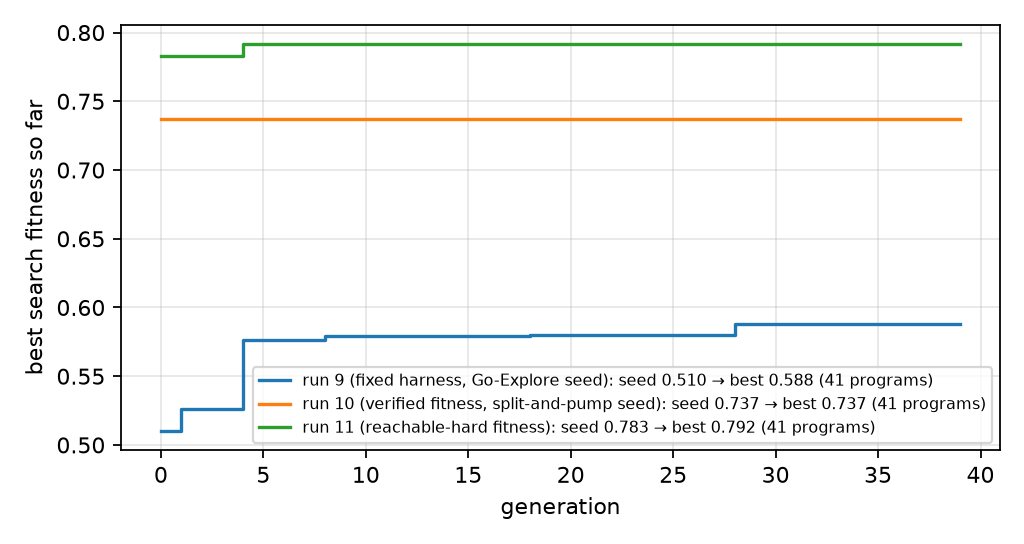
\includegraphics[width=0.52\linewidth]{figures/search_runs_fixed.png}
\caption{Best search fitness by generation on the fixed harness (each run on its own fitness scale). Run 9 (Go-Explore seed) climbs 0.510 $\to$ 0.588; run 10 (verified fitness, split-and-pump seed) never leaves generation 0; run 11 (reachable-hard fitness, same seed) makes its one gain at generation 4 (0.783 $\to$ 0.792) --- the gain that transfers (\S1.3). Every run finds whatever it finds within the first generations.}
\label{fig:fitness}\end{figure}
